\documentclass[tikz,border=5pt,10pt]{standalone}
\usepackage{tikz}
\usetikzlibrary{calc}
\usepackage{pgf,xcolor}
\usepackage{eulervm}
\usepackage{booktabs,rotating,multirow,caption}
\usepackage{makecell}
\usetikzlibrary{automata}
\usetikzlibrary{arrows}
\usepackage{mathdots}
\usetikzlibrary{decorations.pathreplacing}
\usetikzlibrary{backgrounds}
\begin{document}
  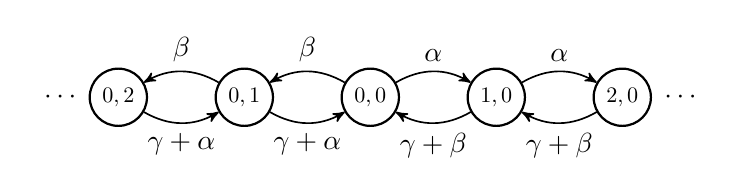
\begin{tikzpicture}[->, >=stealth', auto, semithick, node distance=2cm]
    \tikzstyle{every state}=[fill=white,draw=black,thick,text=black,scale=0.8]
    \node[state]    (0_0)				{$0,0$};
    \node[state]    (1_0)[right of=0_0]	{$1,0$};
    \node[state]    (2_0)[right of=1_0]	{$2,0$};
    \node[state]    (0_1)[left of=0_0]	{$0,1$};
    \node[state]    (0_2)[left of=0_1]	{$0,2$};
    \node[state, draw=none]    (i_0)[right of=2_0, xshift=-1cm]	{$ $};
    \node[state, draw=none]    (0_i)[left of=0_2, xshift=1cm]	{$ $};
    \path
    (0_0)
      edge[bend left]	node{$\alpha$} 			(1_0)
      edge[bend right] 	node[above]{$\beta$}	(0_1)
    (1_0)
      edge[bend left] 	node{$\alpha$}			(2_0)
      edge[bend left] 	node{$\gamma + \beta$}	(0_0)
    (2_0)
      edge[bend left]	node{$\gamma + \beta$}  (1_0)
      edge[draw=none, right]		node{$\cdots$}  		(i_0)
    (0_1)
      edge[bend right]  node[below]{$\gamma + \alpha$}	(0_0)
      edge[bend right]  node[above]{$\beta$}          	(0_2)
    (0_2)
      edge[bend right]  node[below]{$\gamma + \alpha$} 	(0_1)
      edge[draw=none, left]		node[auto=false]{$\cdots$}  	(0_i);
%   \node[above=0.5cm] (A){Patch G};
%   \draw[red] ($(D)+(-1.5,0)$) ellipse (2cm and 3.5cm)node[yshift=3cm]{Patch H};
  \end{tikzpicture}
\end{document}